\documentclass{article}

\usepackage[a4paper, total={6.5in, 11in}]{geometry}
\usepackage{graphicx}
\usepackage{subfig}
\graphicspath{{titech/CSC.T463.ComputerGraphics/h3/}}

\usepackage{latex/common}

\title{Computer Graphics 2021 - Assignment 3}
\author{Sixue Wang\\21M30927\\Tokyo Institute of Technology}

\begin{document}

\maketitle

\section{}
\subsection{Case 1}
First of all, we use a handcrafted 512x512 picture to show aliasing, so we can describe frequency more precisely. The original picture is composed of 34x34 small squares, then the frequency of the original picture in x-axis and y-axis are both $\frac{1}{17}$. On the other hand, the sampling frequency is $\frac{sampling interval}{512}$. The picture has hardly changed when $sampling interval = 3$. Even if the size of small rectangles are changed when $sampling interval = 14$, but it is still composed of 34x34 rectangles. However, the picture will be composed of 30x30 rectangles when $sampling interval = 16$. It could be explained by Nyquist frequency: $2*\frac{sampling interval}{512}=\frac{32}{512}=\frac{1}{16}>\frac{1}{17}$

\begin{figure}[h]
  \begin{tabular}{cc}
    \subfloat[sampling interval = 0]{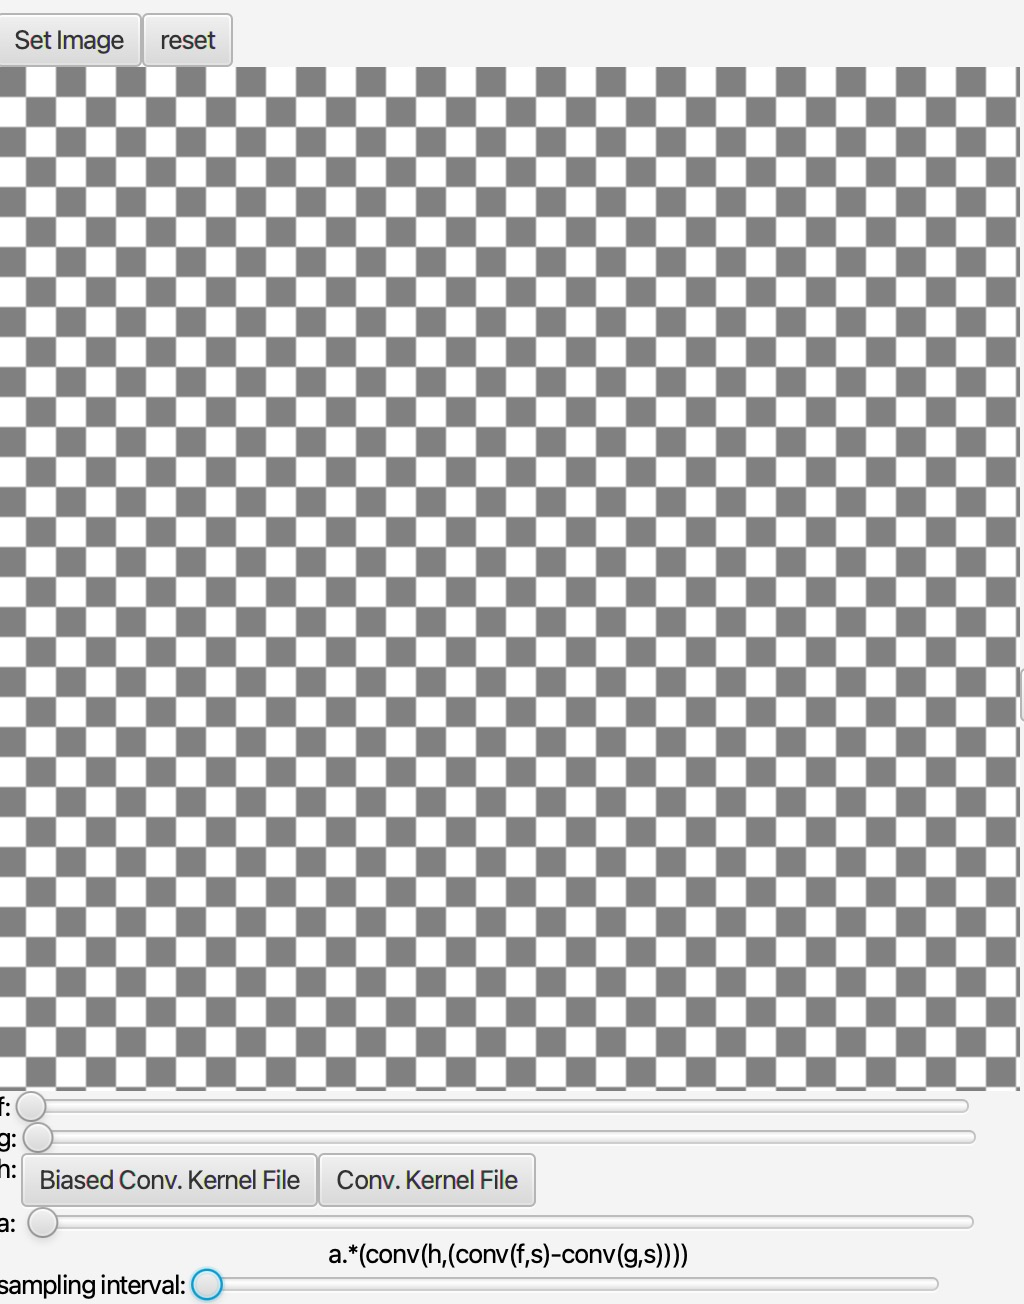
\includegraphics[width=0.3\textwidth]{a-0.png}} &
    \subfloat[sampling interval = 3]{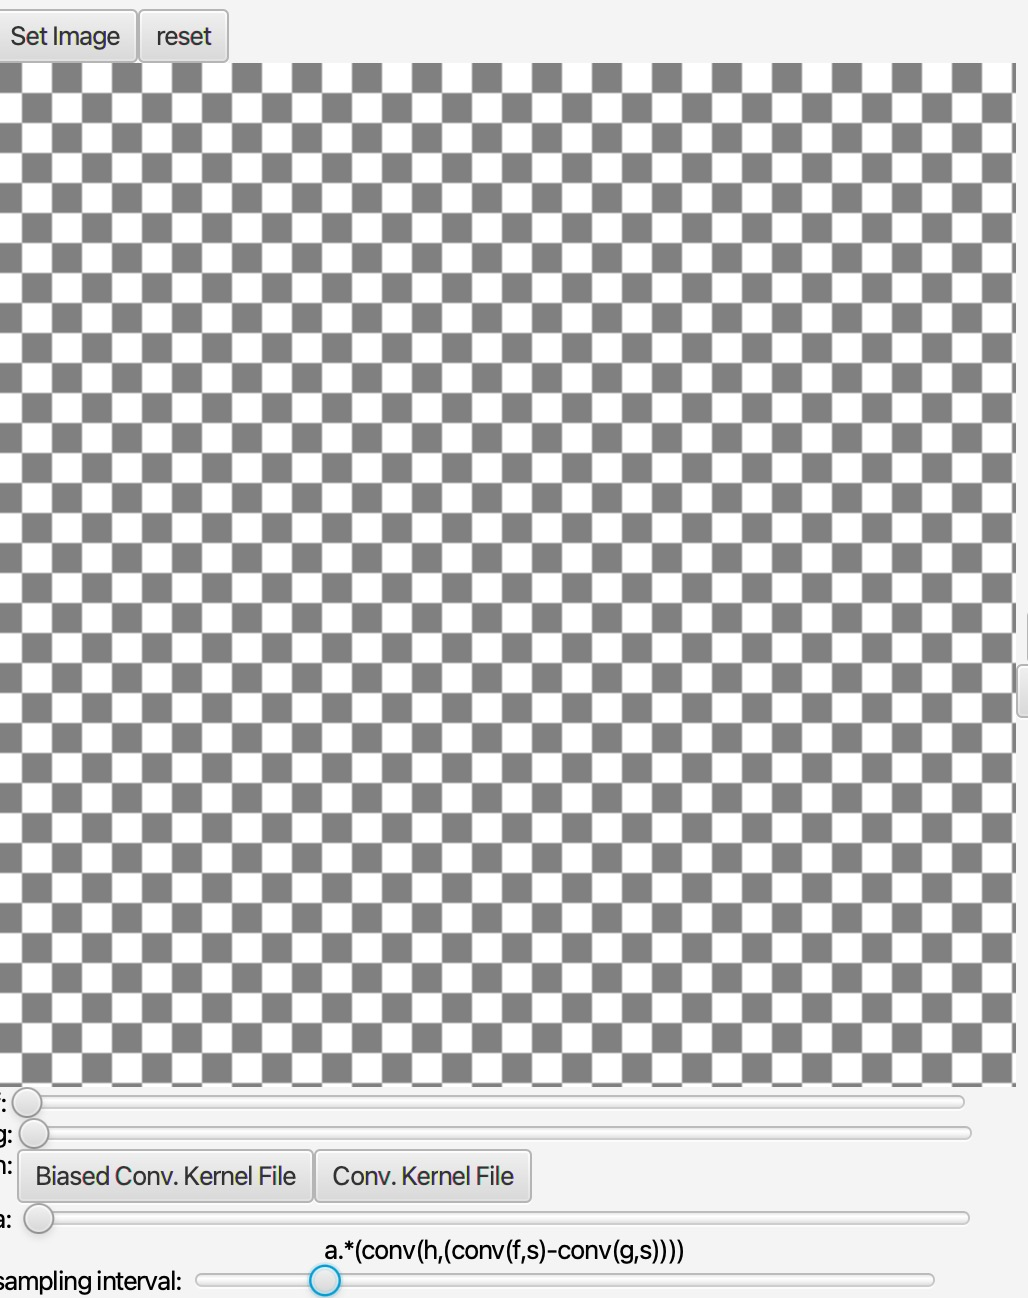
\includegraphics[width=0.3\textwidth]{a-3.png}} \\
    \subfloat[sampling interval = 14]{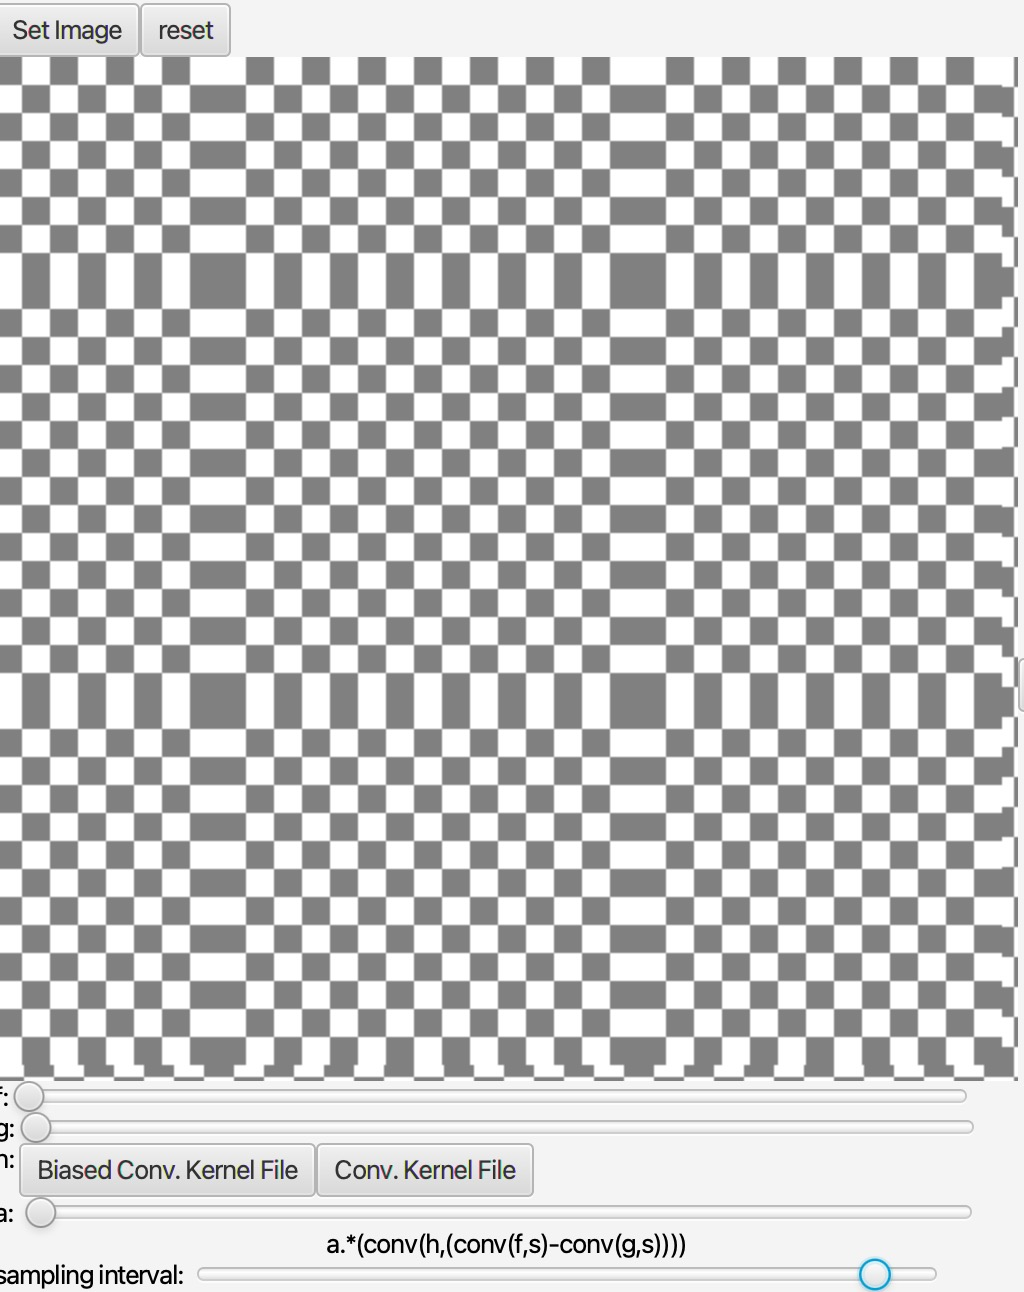
\includegraphics[width=0.3\textwidth]{a-14.png}} &
    \subfloat[sampling interval = 16]{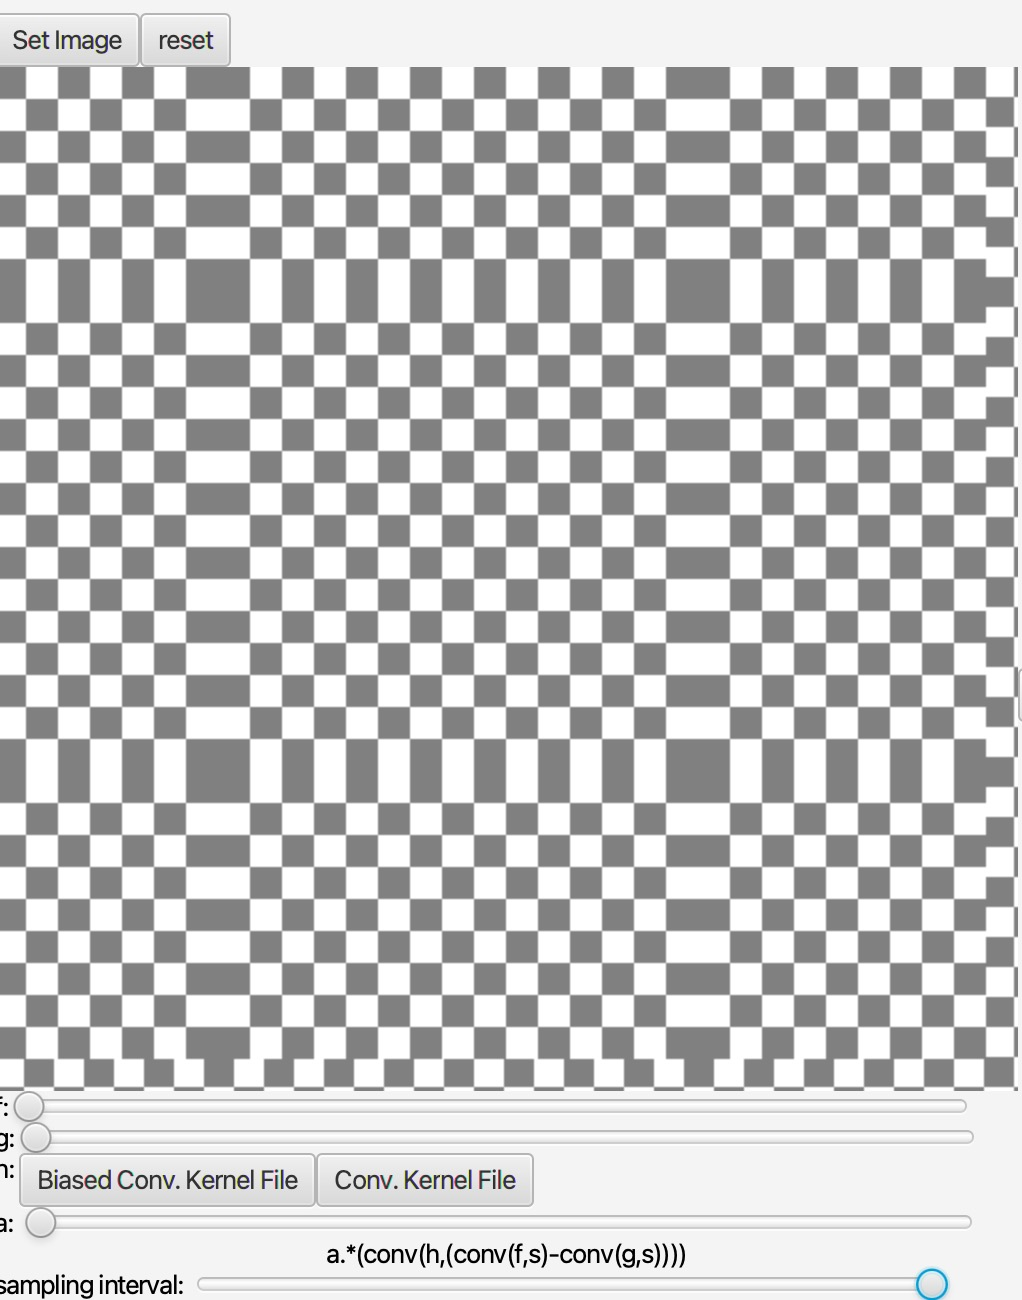
\includegraphics[width=0.3\textwidth]{a-16.png}} \\
  \end{tabular}
\end{figure}

\newpage

\subsection{Case 2}
Now we consider a real picture. Usually, we cannot accurately evaluate the frequency of real pictures, but if the texture is more complex, the frequency will be higher. So the firework pattern in the background will first become blurred even when $sampling interval = 3$. At this time, the text ``Happy New Year 2021'' can still be seen clearly. Then nothing can be distinguished when $sampling interval = 16$.

\begin{figure}[h]
  \begin{tabular}{cc}
    \subfloat[sampling interval = 0]{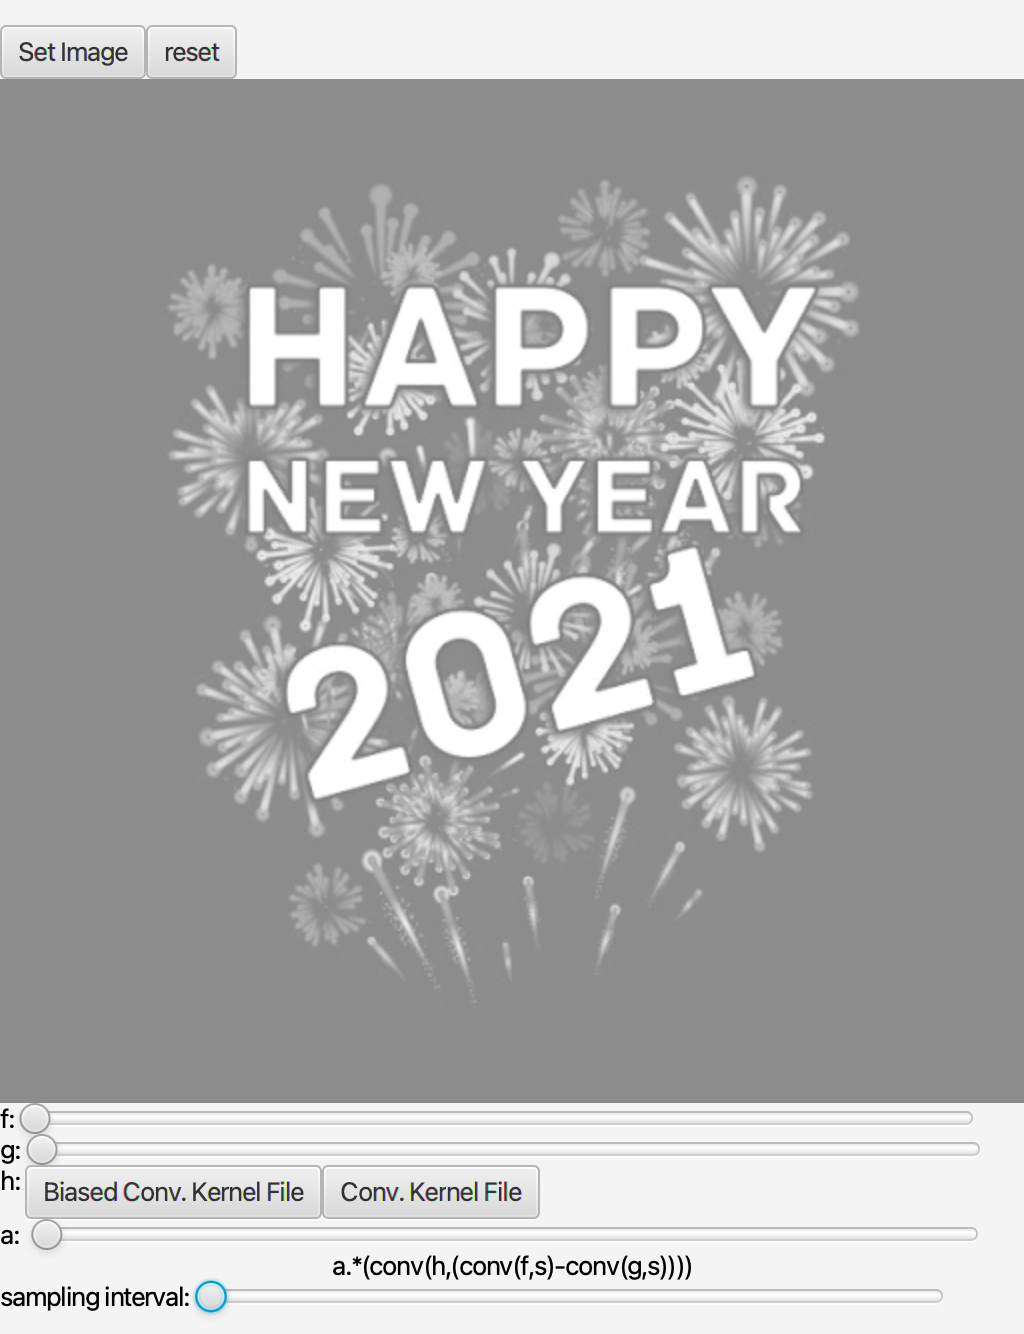
\includegraphics[width=0.3\textwidth]{b-0.png}} &
    \subfloat[sampling interval = 3]{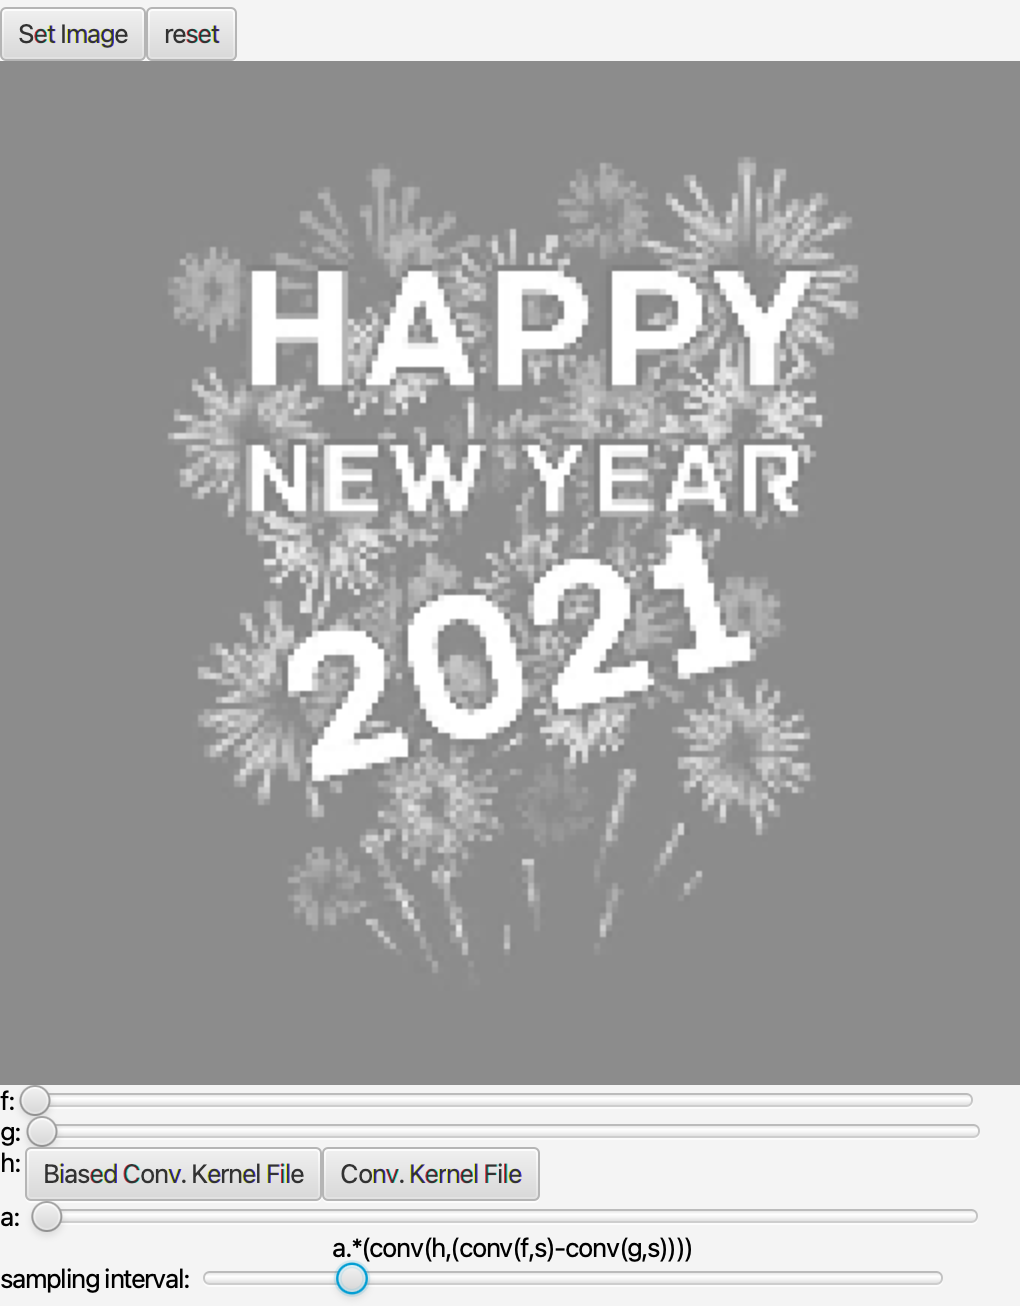
\includegraphics[width=0.3\textwidth]{b-3.png}} \\
    \subfloat[sampling interval = 7]{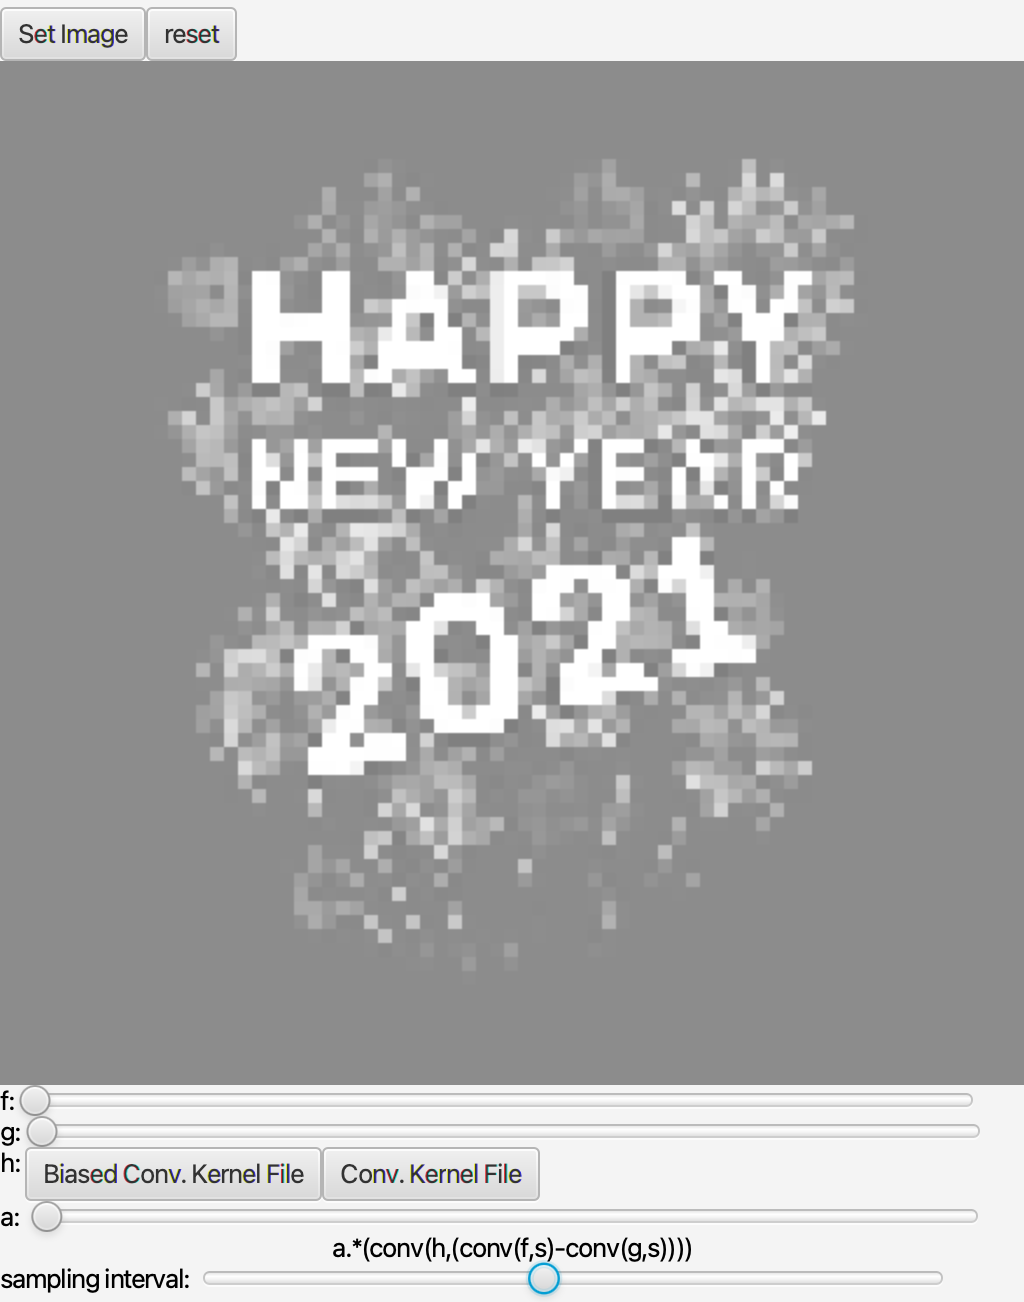
\includegraphics[width=0.3\textwidth]{b-7.png}} &
    \subfloat[sampling interval = 16]{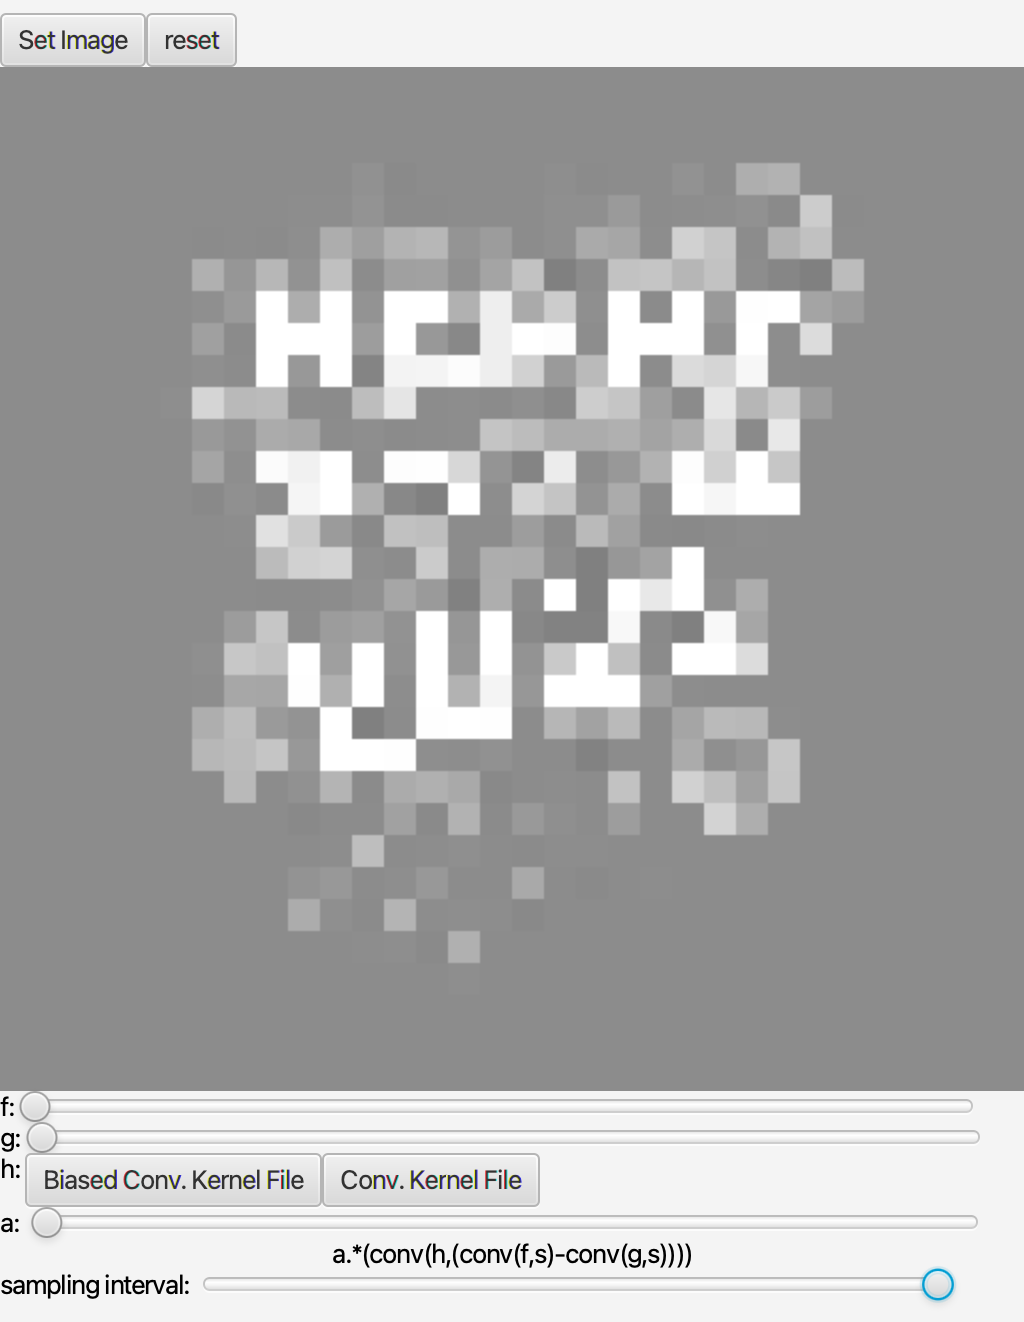
\includegraphics[width=0.3\textwidth]{b-16.png}} \\
  \end{tabular}
\end{figure}

\newpage

\section{}

One of the basic anti-aliasing techniques is applying a low pass filter because aliasing means the overlapping in the high-frequency component. In our case, we use a 3x3 gaussian filter($\sigma=1$)

\begin{figure}[h]
\begin{tabular}{cc}
\subfloat[signal]{
$
\begin{bmatrix}
  0.09486166 & 0.11857707 & 0.09486166 \\
  0.11857707 & 0.14624505 & 0.11857707 \\
  0.09486166 & 0.11857707 & 0.09486166
\end{bmatrix}
$} &
\subfloat[frequency]{
$
\begin{bmatrix}
  0.00543536 & 0.07372493 & 0.00543536 \\
 0.07372493  & 1.         & 0.07372493 \\
 0.00543536  & 0.07372493 & 0.00543536
\end{bmatrix}
$}
\end{tabular}
\end{figure}

%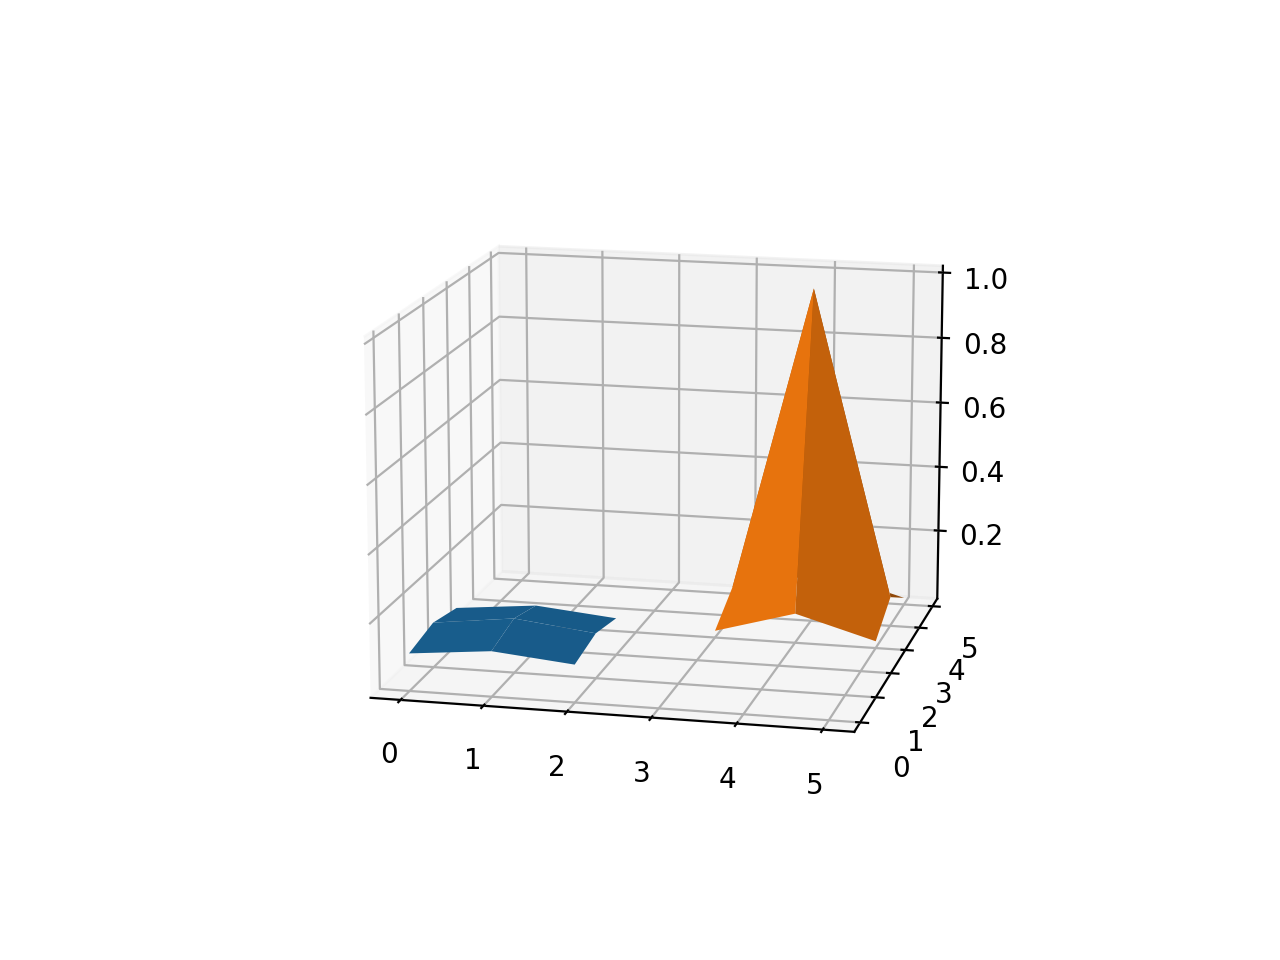
\includegraphics[width=0.5\textwidth]{c-5.png}

As we already know that the FFT of one gaussian is another gaussian, convolution with this filter in the signal domain means multiplication on in the frequency domain. So we apply this filter before sampling to remove high-frequenc component. Now let's compare the above picture when $sampling filter = 3$, the processed picture is much better than the original one.

\begin{figure}[h]
  \begin{tabular}{cc}
    \subfloat[without filter]{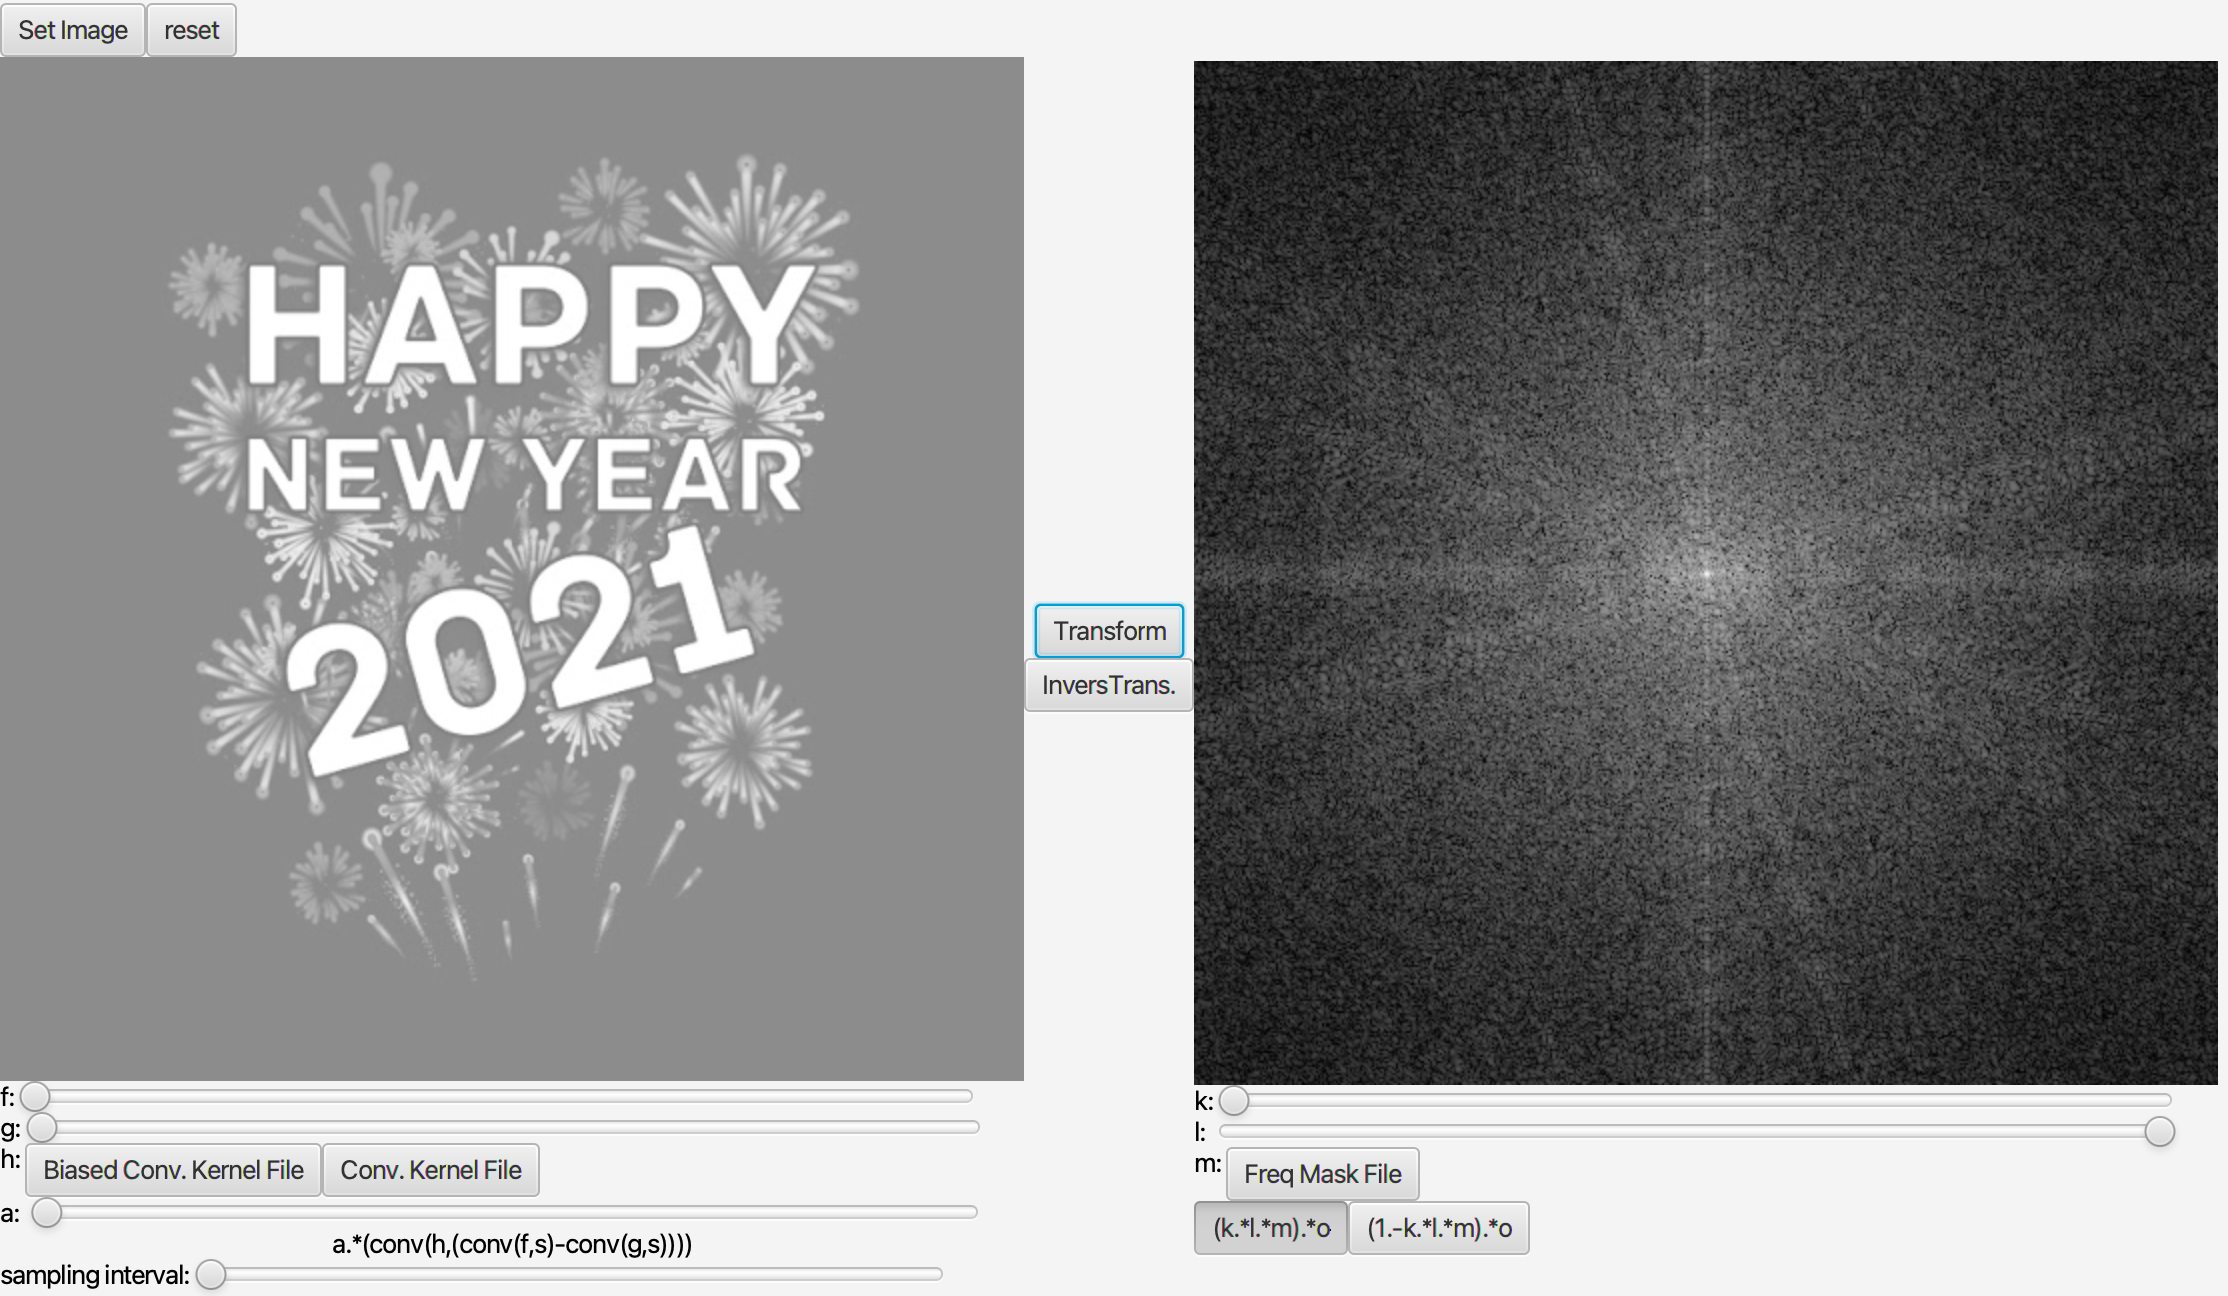
\includegraphics[width=0.4\textwidth]{c-0.png}} &
    \subfloat[with filter]{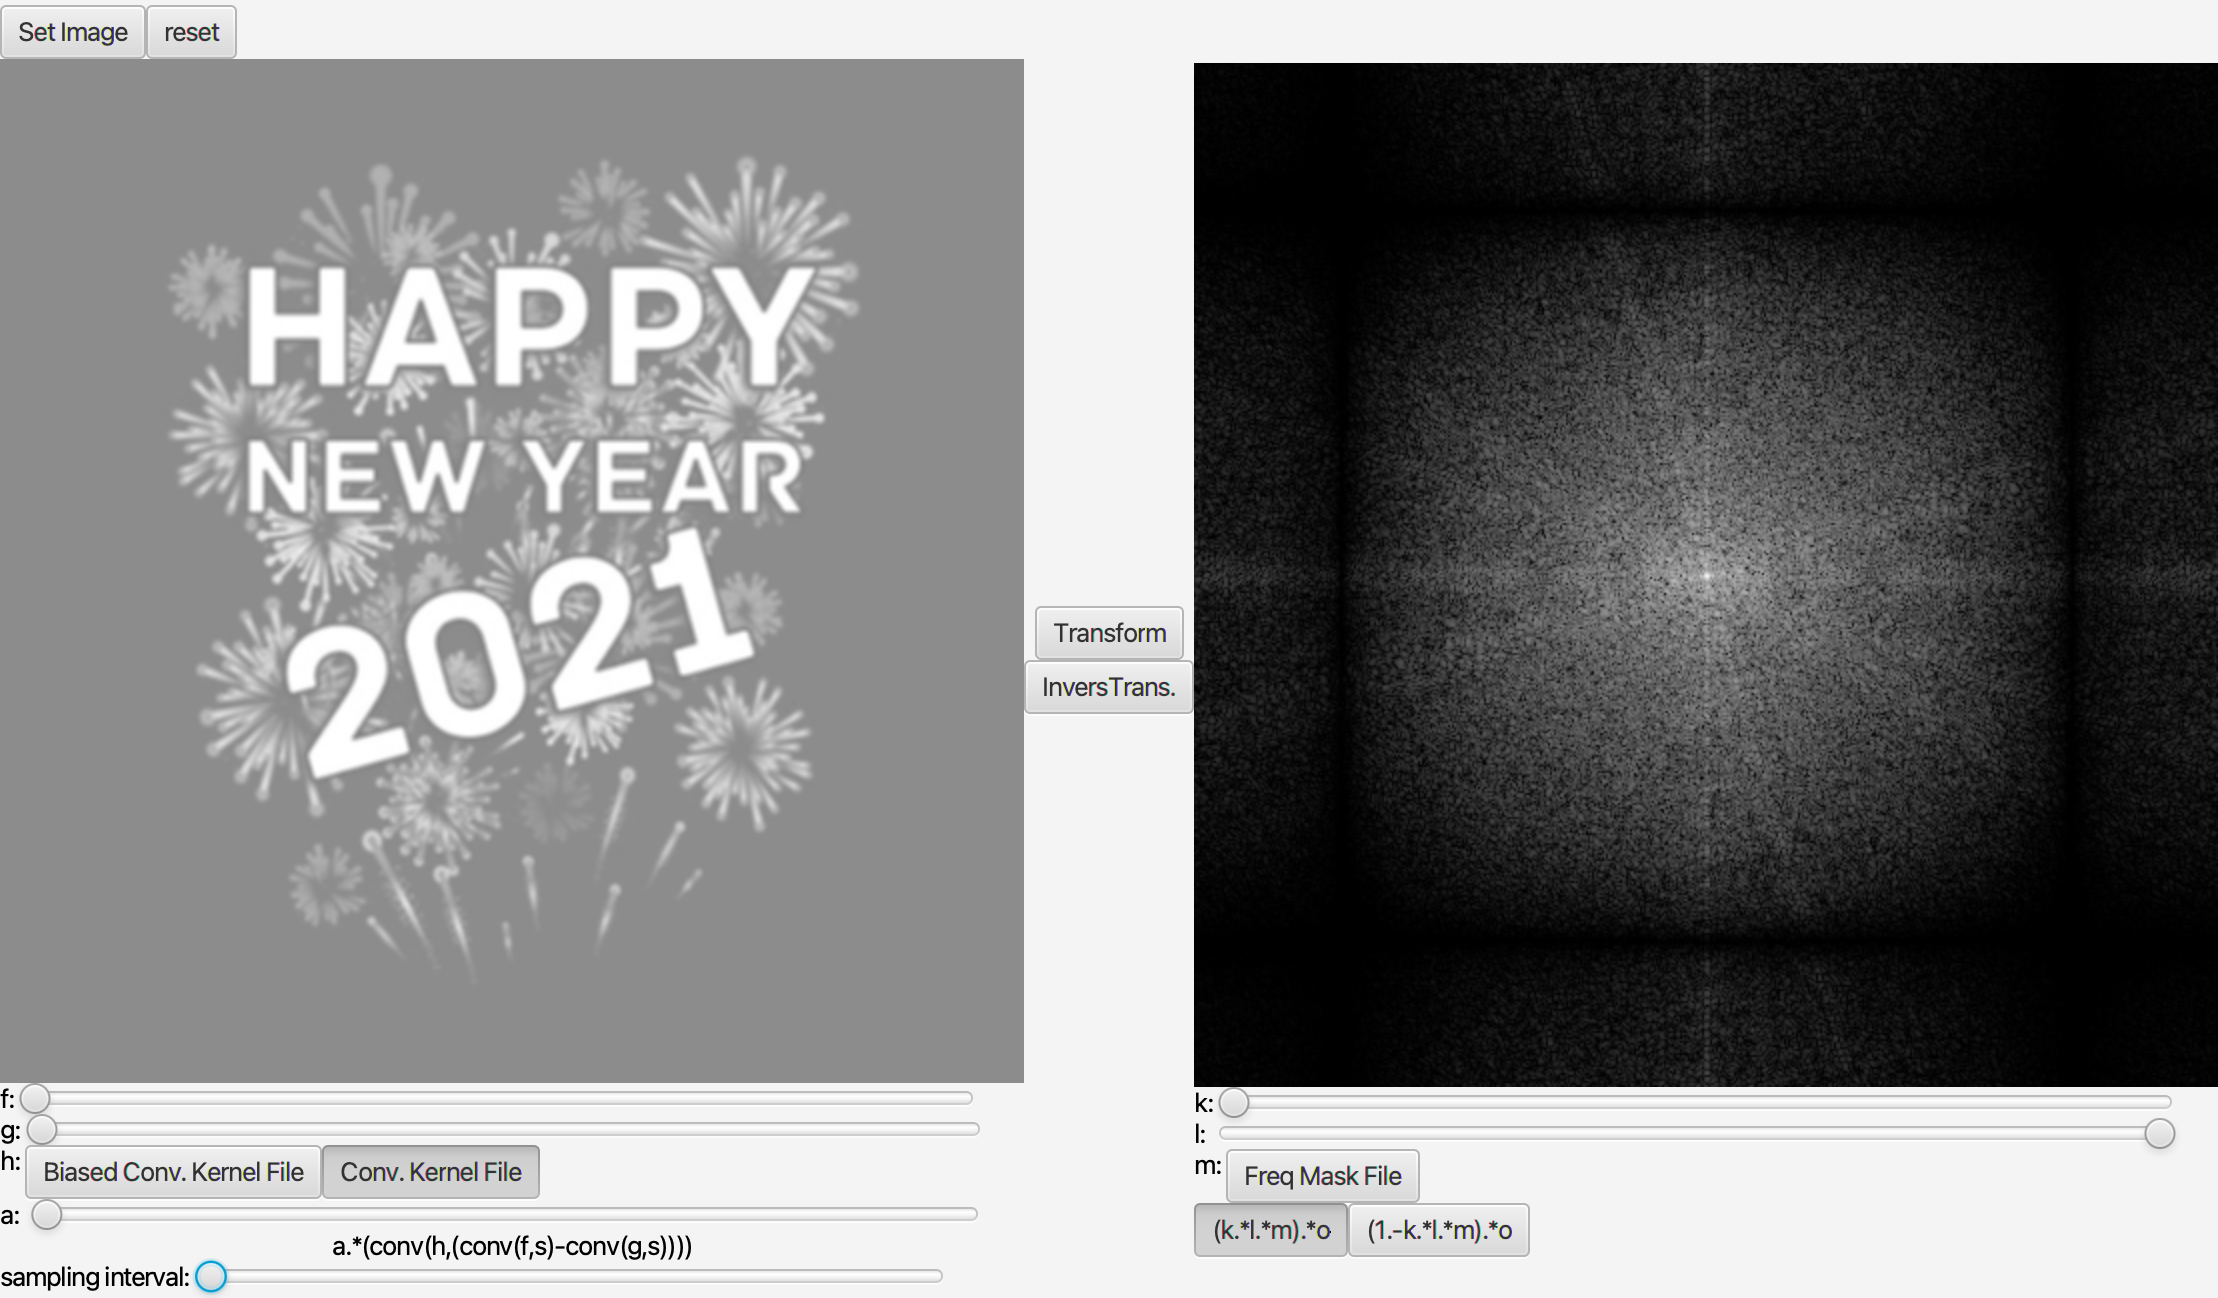
\includegraphics[width=0.4\textwidth]{c-3.png}} \\
    \subfloat[without filter]{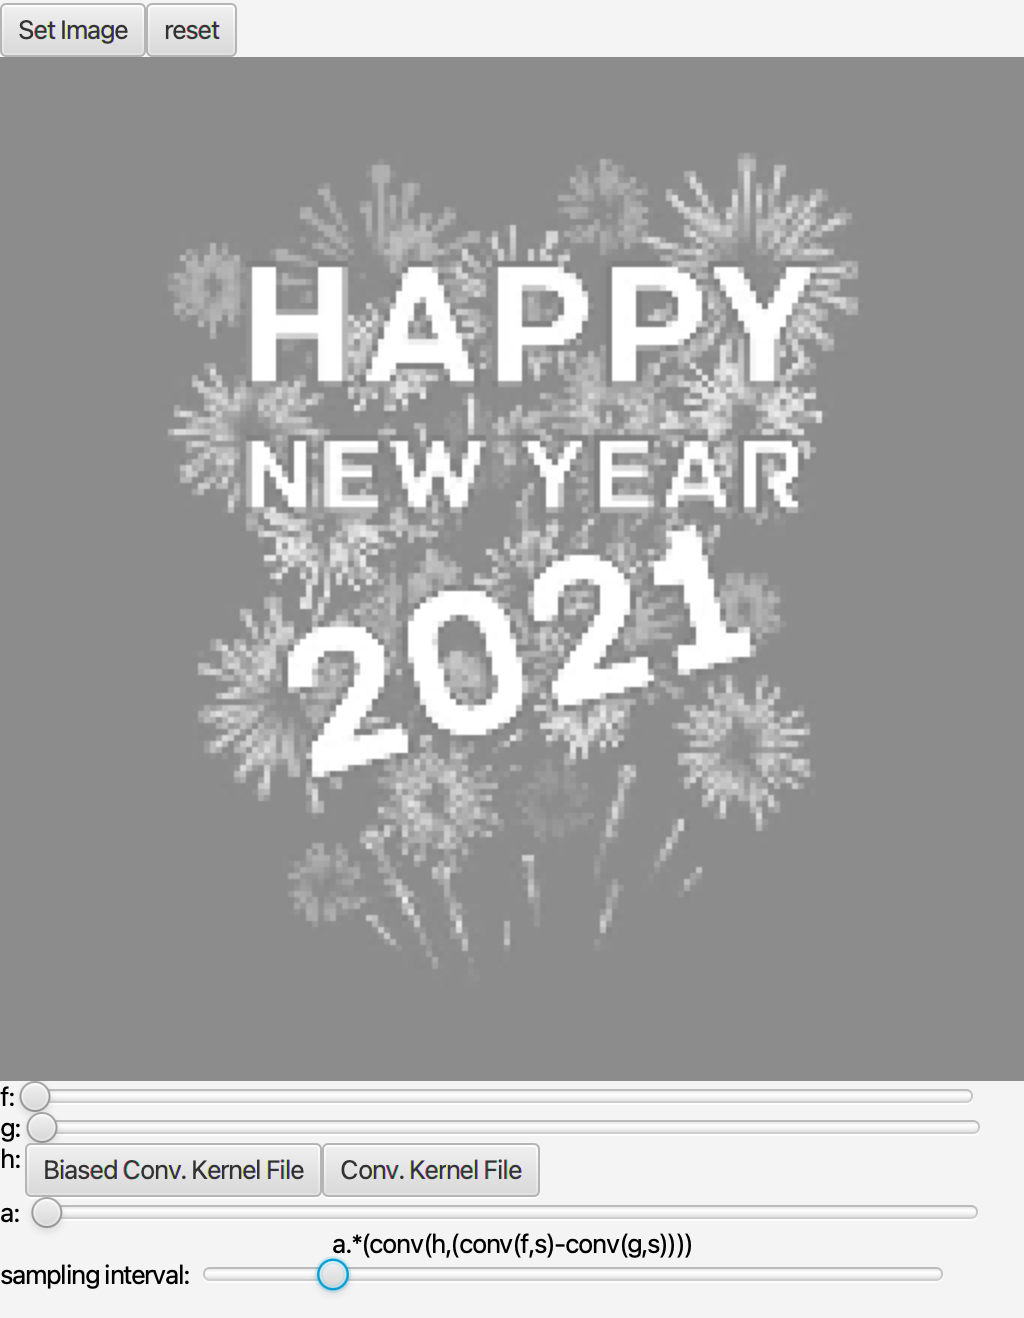
\includegraphics[width=0.3\textwidth]{c-1.png}} &
    \subfloat[with filter]{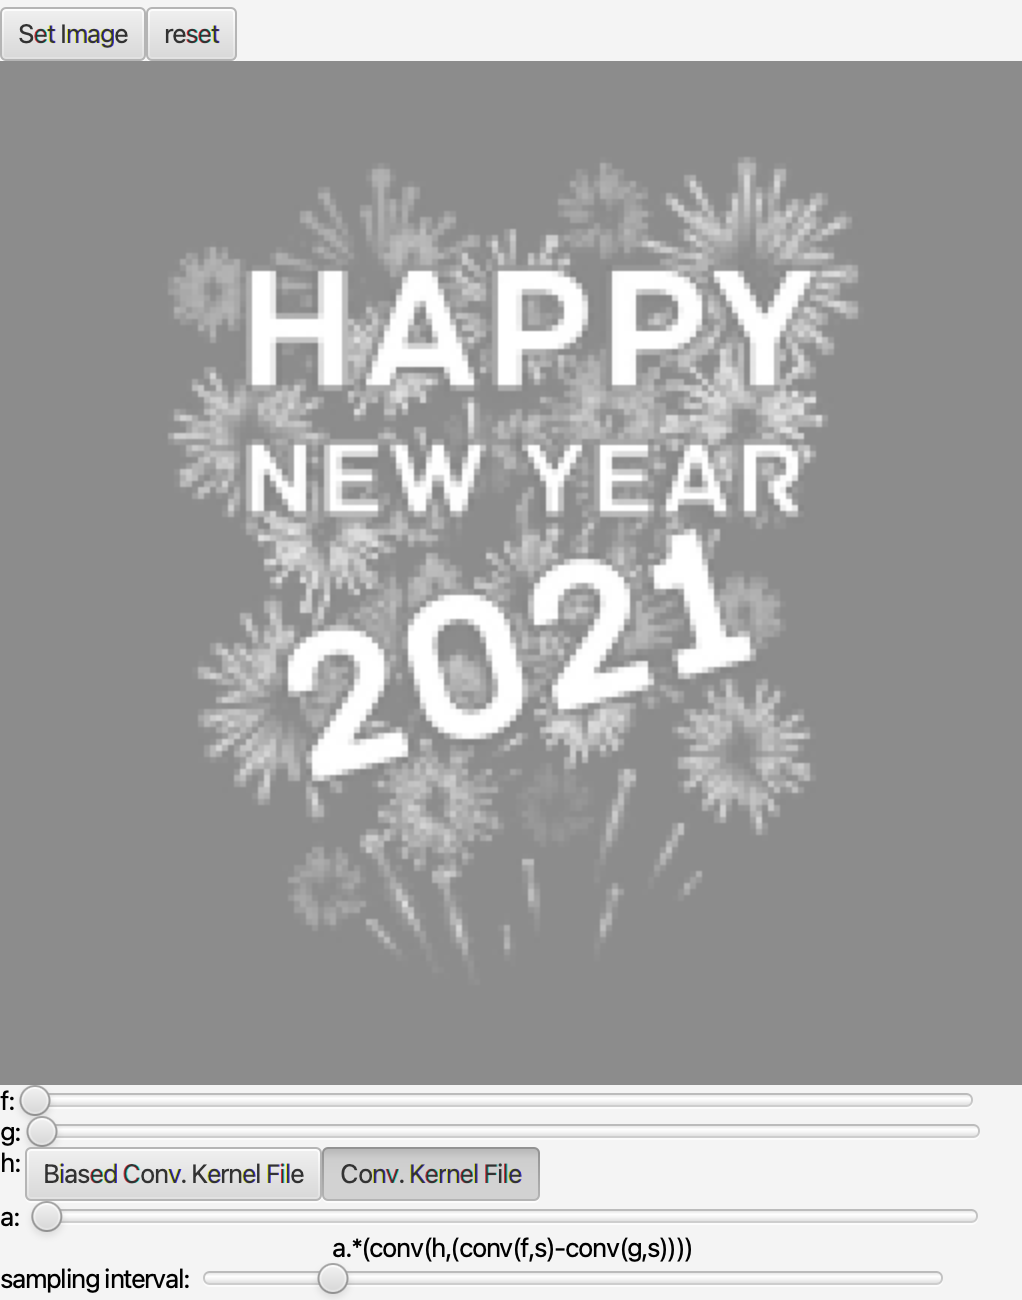
\includegraphics[width=0.3\textwidth]{c-2.png}}
  \end{tabular}
\end{figure}



\end{document}
